% ----------------------------------------------------------------------
%
%                            TFMTesis.tex
%
%----------------------------------------------------------------------
%
% Este fichero contiene el "documento maestro" del documento. Lo único
% que hace es configurar el entorno LaTeX e incluir los ficheros .tex
% que contienen cada sección.
%
%----------------------------------------------------------------------
%
% Los ficheros necesarios para este documento son:
%
%       TeXiS/* : ficheros de la plantilla TeXiS.
%       Cascaras/* : ficheros con las partes del documento que no
%          son capítulos ni apéndices (portada, agradecimientos, etc.)
%       Capitulos/*.tex : capítulos de la tesis
%       Apendices/*.tex: apéndices de la tesis
%       constantes.tex: constantes LaTeX
%       config.tex : configuración de la "compilación" del documento
%       guionado.tex : palabras con guiones
%
% Para la bibliografía, además, se necesitan:
%
%       *.bib : ficheros con la información de las referencias
%
% ---------------------------------------------------------------------

\documentclass[12pt,a4paper,twoside]{book}

%
% Definimos  el   comando  \compilaCapitulo,  que   luego  se  utiliza
% (opcionalmente) en config.tex. Quedaría  mejor si también se definiera
% en  ese fichero,  pero por  el modo  en el  que funciona  eso  no es
% posible. Puedes consultar la documentación de ese fichero para tener
% más  información. Definimos también  \compilaApendice, que  tiene el
% mismo  cometido, pero  que se  utiliza para  compilar  únicamente un
% apéndice.
%
%
% Si  queremos   compilar  solo   una  parte  del   documento  podemos
% especificar mediante  \includeonly{...} qué ficheros  son los únicos
% que queremos  que se incluyan.  Esto  es útil por  ejemplo para sólo
% compilar un capítulo.
%
% El problema es que todos aquellos  ficheros que NO estén en la lista
% NO   se  incluirán...  y   eso  también   afecta  a   ficheros  de
% la plantilla...
%
% Total,  que definimos  una constante  con los  ficheros  que siempre
% vamos a querer compilar  (aquellos relacionados con configuración) y
% luego definimos \compilaCapitulo.
\newcommand{\ficherosBasicosTeXiS}{%
TeXiS/TeXiS_pream,TeXiS/TeXiS_cab,TeXiS/TeXiS_bib,TeXiS/TeXiS_cover%
}
\newcommand{\ficherosBasicosTexto}{%
constantes,guionado,Cascaras/bibliografia,config%
}
\newcommand{\compilaCapitulo}[1]{%
\includeonly{\ficherosBasicosTeXiS,\ficherosBasicosTexto,Capitulos/#1}%
}

\newcommand{\compilaApendice}[1]{%
\includeonly{\ficherosBasicosTeXiS,\ficherosBasicosTexto,Apendices/#1}%
}

%- - - - - - - - - - - - - - - - - - - - - - - - - - - - - - - - - - -
%            Preámbulo del documento. Configuraciones varias
%- - - - - - - - - - - - - - - - - - - - - - - - - - - - - - - - - - -

% Define  el  tipo  de  compilación que  estamos  haciendo.   Contiene
% definiciones  de  constantes que  cambian  el  comportamiento de  la
% compilación. Debe incluirse antes del paquete TeXiS/TeXiS.sty
%---------------------------------------------------------------------
%
%                          config.tex
%
%---------------------------------------------------------------------
%
% Contiene la  definición de constantes  que determinan el modo  en el
% que se compilará el documento.
%
%---------------------------------------------------------------------
%
% En concreto, podemos  indicar si queremos "modo release",  en el que
% no  aparecerán  los  comentarios  (creados  mediante  \com{Texto}  o
% \comp{Texto}) ni los "por  hacer" (creados mediante \todo{Texto}), y
% sí aparecerán los índices. El modo "debug" (o mejor dicho en modo no
% "release" muestra los índices  (construirlos lleva tiempo y son poco
% útiles  salvo  para   la  versión  final),  pero  sí   el  resto  de
% anotaciones.
%
% Si se compila con LaTeX (no  con pdflatex) en modo Debug, también se
% muestran en una esquina de cada página las entradas (en el índice de
% palabras) que referencian  a dicha página (consulta TeXiS_pream.tex,
% en la parte referente a show).
%
% El soporte para  el índice de palabras en  TeXiS es embrionario, por
% lo  que no  asumas que  esto funcionará  correctamente.  Consulta la
% documentación al respecto en TeXiS_pream.tex.
%
%
% También  aquí configuramos  si queremos  o  no que  se incluyan  los
% acrónimos  en el  documento final  en la  versión release.  Para eso
% define (o no) la constante \acronimosEnRelease.
%
% Utilizando \compilaCapitulo{nombre}  podemos también especificar qué
% capítulo(s) queremos que se compilen. Si no se pone nada, se compila
% el documento  completo.  Si se pone, por  ejemplo, 01Introduccion se
% compilará únicamente el fichero Capitulos/01Introduccion.tex
%
% Para compilar varios  capítulos, se separan sus nombres  con comas y
% no se ponen espacios de separación.
%
% En realidad  la macro \compilaCapitulo  está definida en  el fichero
% principal tesis.tex.
%
%---------------------------------------------------------------------


% Comentar la línea si no se compila en modo release.
% TeXiS hará el resto.
% ¡¡¡Si cambias esto, haz un make clean antes de recompilar!!!
\def\release{1}


% Descomentar la linea si se quieren incluir los
% acrónimos en modo release (en modo debug
% no se incluirán nunca).
% ¡¡¡Si cambias esto, haz un make clean antes de recompilar!!!
%\def\acronimosEnRelease{1}


% Descomentar la línea para establecer el capítulo que queremos
% compilar

% \compilaCapitulo{01Introduccion}
% \compilaCapitulo{02EstructuraYGeneracion}
% \compilaCapitulo{03Edicion}
% \compilaCapitulo{04Imagenes}
% \compilaCapitulo{05Bibliografia}
% \compilaCapitulo{06Makefile}

% \compilaApendice{01AsiSeHizo}

% Variable local para emacs, para  que encuentre el fichero maestro de
% compilación y funcionen mejor algunas teclas rápidas de AucTeX
%%%
%%% Local Variables:
%%% mode: latex
%%% TeX-master: "./Tesis.tex"
%%% End:


% Paquete de la plantilla
\usepackage{TeXiS/TeXiS}

% Incluimos el fichero con comandos de constantes
%---------------------------------------------------------------------
%
%                          constantes.tex
%
%---------------------------------------------------------------------
%
% Fichero que  declara nuevos comandos LaTeX  sencillos realizados por
% comodidad en la escritura de determinadas palabras
%
%---------------------------------------------------------------------

%%%%%%%%%%%%%%%%%%%%%%%%%%%%%%%%%%%%%%%%%%%%%%%%%%%%%%%%%%%%%%%%%%%%%%
% Comando: 
%
%       \titulo
%
% Resultado: 
%
% Escribe el título del documento.
%%%%%%%%%%%%%%%%%%%%%%%%%%%%%%%%%%%%%%%%%%%%%%%%%%%%%%%%%%%%%%%%%%%%%%
\def\titulo{\textsc{TeXiS}: Una plantilla de \LaTeX\
  para Tesis y otros documentos}

%%%%%%%%%%%%%%%%%%%%%%%%%%%%%%%%%%%%%%%%%%%%%%%%%%%%%%%%%%%%%%%%%%%%%%
% Comando: 
%
%       \autor
%
% Resultado: 
%
% Escribe el autor del documento.
%%%%%%%%%%%%%%%%%%%%%%%%%%%%%%%%%%%%%%%%%%%%%%%%%%%%%%%%%%%%%%%%%%%%%%
\def\autor{Marco Antonio y Pedro Pablo G\'omez Mart\'in}

% Variable local para emacs, para  que encuentre el fichero maestro de
% compilación y funcionen mejor algunas teclas rápidas de AucTeX

%%%
%%% Local Variables:
%%% mode: latex
%%% TeX-master: "tesis.tex"
%%% End:


% Sacamos en el log de la compilación el copyright
%\typeout{Copyright Marco Antonio and Pedro Pablo Gomez Martin}

%
% "Metadatos" para el PDF
%
\ifpdf\hypersetup{%
    pdftitle = {\titulo},
    pdfsubject = {Plantilla de Tesis},
    pdfauthor = {\textcopyright\ \autor},
    pdfcreator = {\LaTeX\ con el paquete \flqq hyperref\frqq},
    pdfproducer = {pdfeTeX-0.\the\pdftexversion\pdftexrevision},
    colorlinks, 
    citecolor=[HTML]{6f03fc}, 
    filecolor=black, 
    linkcolor=blue, 
    urlcolor=blue
    }
    \pdfinfo{/CreationDate (\today)}
\fi


%- - - - - - - - - - - - - - - - - - - - - - - - - - - - - - - - - - -
%                        Documento
%- - - - - - - - - - - - - - - - - - - - - - - - - - - - - - - - - - -
\begin{document}

% Incluimos el  fichero de definición de guionado  de algunas palabras
% que LaTeX no ha dividido como debería
%----------------------------------------------------------------
%
%                          guionado.tex
%
%----------------------------------------------------------------
%
% Fichero con algunas divisiones de palabras que LaTeX no
% hace correctamente si no se le da alguna ayuda.
%
%----------------------------------------------------------------

\hyphenation{
% a
abs-trac-to
abs-trac-tos
abs-trac-ta
abs-trac-tas
ac-tua-do-res
a-gra-de-ci-mien-tos
ana-li-za-dor
an-te-rio-res
an-te-rior-men-te
apa-rien-cia
a-pro-pia-do
a-pro-pia-dos
a-pro-pia-da
a-pro-pia-das
a-pro-ve-cha-mien-to
a-que-llo
a-que-llos
a-que-lla
a-que-llas
a-sig-na-tu-ra
a-sig-na-tu-ras
a-so-cia-da
a-so-cia-das
a-so-cia-do
a-so-cia-dos
au-to-ma-ti-za-do
% b
batch
bi-blio-gra-fía
bi-blio-grá-fi-cas
bien
bo-rra-dor
boo-l-ean-expr
% c
ca-be-ce-ra
call-me-thod-ins-truc-tion
cas-te-lla-no
cir-cuns-tan-cia
cir-cuns-tan-cias
co-he-ren-te
co-he-ren-tes
co-he-ren-cia
co-li-bri
co-men-ta-rio
co-mer-cia-les
co-no-ci-mien-to
cons-cien-te
con-si-de-ra-ba
con-si-de-ra-mos
con-si-de-rar-se
cons-tan-te
cons-trucción
cons-tru-ye
cons-tru-ir-se
con-tro-le
co-rrec-ta-men-te
co-rres-pon-den
co-rres-pon-dien-te
co-rres-pon-dien-tes
co-ti-dia-na
co-ti-dia-no
crean
cris-ta-li-zan
cu-rri-cu-la
cu-rri-cu-lum
cu-rri-cu-lar
cu-rri-cu-la-res
% d
de-di-ca-do
de-di-ca-dos
de-di-ca-da
de-di-ca-das
de-rro-te-ro
de-rro-te-ros
de-sa-rro-llo
de-sa-rro-llos
de-sa-rro-lla-do
de-sa-rro-lla-dos
de-sa-rro-lla-da
de-sa-rro-lla-das
de-sa-rro-lla-dor
de-sa-rro-llar
des-cri-bi-re-mos
des-crip-ción
des-crip-cio-nes
des-cri-to
des-pués
de-ta-lla-do
de-ta-lla-dos
de-ta-lla-da
de-ta-lla-das
di-a-gra-ma
di-a-gra-mas
di-se-ños
dis-po-ner
dis-po-ni-bi-li-dad
do-cu-men-ta-da
do-cu-men-to
do-cu-men-tos
% e
edi-ta-do
e-du-ca-ti-vo
e-du-ca-ti-vos
e-du-ca-ti-va
e-du-ca-ti-vas
e-la-bo-ra-do
e-la-bo-ra-dos
e-la-bo-ra-da
e-la-bo-ra-das
es-co-llo
es-co-llos
es-tu-dia-do
es-tu-dia-dos
es-tu-dia-da
es-tu-dia-das
es-tu-dian-te
e-va-lua-cio-nes
e-va-lua-do-res
exis-ten-tes
exhaus-ti-va
ex-pe-rien-cia
ex-pe-rien-cias
% f
for-ma-li-za-do
% g
ge-ne-ra-ción
ge-ne-ra-dor
ge-ne-ra-do-res
ge-ne-ran
% h
he-rra-mien-ta
he-rra-mien-tas
% i
i-dio-ma
i-dio-mas
im-pres-cin-di-ble
im-pres-cin-di-bles
in-de-xa-do
in-de-xa-dos
in-de-xa-da
in-de-xa-das
in-di-vi-dual
in-fe-ren-cia
in-fe-ren-cias
in-for-ma-ti-ca
in-gre-dien-te
in-gre-dien-tes
in-me-dia-ta-men-te
ins-ta-la-do
ins-tan-cias
% j
% k
% l
len-gua-je
li-be-ra-to-rio
li-be-ra-to-rios
li-be-ra-to-ria
li-be-ra-to-rias
li-mi-ta-do
li-te-ra-rio
li-te-ra-rios
li-te-ra-ria
li-te-ra-rias
lo-tes
% m
ma-ne-ra
ma-nual
mas-que-ra-de
ma-yor
me-mo-ria
mi-nis-te-rio
mi-nis-te-rios
mo-de-lo
mo-de-los
mo-de-la-do
mo-du-la-ri-dad
mo-vi-mien-to
% n
na-tu-ral
ni-vel
nues-tro
% o
obs-tan-te
o-rien-ta-do
o-rien-ta-dos
o-rien-ta-da
o-rien-ta-das
% p
pa-ra-le-lo
pa-ra-le-la
par-ti-cu-lar
par-ti-cu-lar-men-te
pe-da-gó-gi-ca
pe-da-gó-gi-cas
pe-da-gó-gi-co
pe-da-gó-gi-cos
pe-rio-di-ci-dad
per-so-na-je
plan-te-a-mien-to
plan-te-a-mien-tos
po-si-ción
pre-fe-ren-cia
pre-fe-ren-cias
pres-cin-di-ble
pres-cin-di-bles
pri-me-ra
pro-ble-ma
pro-ble-mas
pró-xi-mo
pu-bli-ca-cio-nes
pu-bli-ca-do
% q
% r
rá-pi-da
rá-pi-do
ra-zo-na-mien-to
ra-zo-na-mien-tos
re-a-li-zan-do
re-fe-ren-cia
re-fe-ren-cias
re-fe-ren-cia-da
re-fe-ren-cian
re-le-van-tes
re-pre-sen-ta-do
re-pre-sen-ta-dos
re-pre-sen-ta-da
re-pre-sen-ta-das
re-pre-sen-tar-lo
re-qui-si-to
re-qui-si-tos
res-pon-der
res-pon-sa-ble
% s
se-pa-ra-do
si-guien-do
si-guien-te
si-guien-tes
si-guie-ron
si-mi-lar
si-mi-la-res
si-tua-ción
% t
tem-pe-ra-ments
te-ner
trans-fe-ren-cia
trans-fe-ren-cias
% u
u-sua-rio
Unreal-Ed
% v
va-lor
va-lo-res
va-rian-te
ver-da-de-ro
ver-da-de-ros
ver-da-de-ra
ver-da-de-ras
ver-da-de-ra-men-te
ve-ri-fi-ca
% w
% x
% y
% z
}
% Variable local para emacs, para que encuentre el fichero
% maestro de compilación
%%%
%%% Local Variables:
%%% mode: latex
%%% TeX-master: "./Tesis.tex"
%%% End:


% Marcamos  el inicio  del  documento para  la  numeración de  páginas
% (usando números romanos para esta primera fase).
\frontmatter
\pagestyle{empty}

%---------------------------------------------------------------------
%
%                          configCover.tex
%
%---------------------------------------------------------------------
%
% cover.tex
% Copyright 2009 Marco Antonio Gomez-Martin, Pedro Pablo Gomez-Martin
%
% This file belongs to the TeXiS manual, a LaTeX template for writting
% Thesis and other documents. The complete last TeXiS package can
% be obtained from http://gaia.fdi.ucm.es/projects/texis/
%
% Although the TeXiS template itself is distributed under the 
% conditions of the LaTeX Project Public License
% (http://www.latex-project.org/lppl.txt), the manual content
% uses the CC-BY-SA license that stays that you are free:
%
%    - to share & to copy, distribute and transmit the work
%    - to remix and to adapt the work
%
% under the following conditions:
%
%    - Attribution: you must attribute the work in the manner
%      specified by the author or licensor (but not in any way that
%      suggests that they endorse you or your use of the work).
%    - Share Alike: if you alter, transform, or build upon this
%      work, you may distribute the resulting work only under the
%      same, similar or a compatible license.
%
% The complete license is available in
% http://creativecommons.org/licenses/by-sa/3.0/legalcode
%
%---------------------------------------------------------------------
%
% Fichero que contiene la configuración de la portada y de la 
% primera hoja del documento.
%
%---------------------------------------------------------------------


% Pueden configurarse todos los elementos del contenido de la portada
% utilizando comandos.

%%%%%%%%%%%%%%%%%%%%%%%%%%%%%%%%%%%%%%%%%%%%%%%%%%%%%%%%%%%%%%%%%%%%%%
% Título del documento:
% \tituloPortada{titulo}
% Nota:
% Si no se define se utiliza el del \titulo. Este comando permite
% cambiar el título de forma que se especifiquen dónde se quieren
% los retornos de carro cuando se utilizan fuentes grandes.
%%%%%%%%%%%%%%%%%%%%%%%%%%%%%%%%%%%%%%%%%%%%%%%%%%%%%%%%%%%%%%%%%%%%%%
\tituloPortada{%
Desarrollo de una aplicación móvil para recomendaciones de hábitos saludables
}


%%%%%%%%%%%%%%%%%%%%%%%%%%%%%%%%%%%%%%%%%%%%%%%%%%%%%%%%%%%%%%%%%%%%%%
% Título del documento en inglés:
% \tituloPortadaEng{titulo}
% Nota:
% Si no se define se utiliza el del \titulo. Este comando permite
% cambiar el título de forma que se especifiquen dónde se quieren
% los retornos de carro cuando se utilizan fuentes grandes.
%%%%%%%%%%%%%%%%%%%%%%%%%%%%%%%%%%%%%%%%%%%%%%%%%%%%%%%%%%%%%%%%%%%%%%
\tituloPortadaEng{%
Development of a mobile application for healthy habits recommendations.
}

%%%%%%%%%%%%%%%%%%%%%%%%%%%%%%%%%%%%%%%%%%%%%%%%%%%%%%%%%%%%%%%%%%%%%%
% Autor del documento:
% \autorPortada{Nombre}
% Se utiliza en la portada y en el valor por defecto del
% primer subtítulo de la segunda portada.
%%%%%%%%%%%%%%%%%%%%%%%%%%%%%%%%%%%%%%%%%%%%%%%%%%%%%%%%%%%%%%%%%%%%%%
\autorPortada{{Rodrigo Souto Santos}}

%%%%%%%%%%%%%%%%%%%%%%%%%%%%%%%%%%%%%%%%%%%%%%%%%%%%%%%%%%%%%%%%%%%%%%
% Fecha de publicación:
% \fechaPublicacion{Fecha}
% Puede ser vacío. Aparece en la última línea de ambas portadas
%%%%%%%%%%%%%%%%%%%%%%%%%%%%%%%%%%%%%%%%%%%%%%%%%%%%%%%%%%%%%%%%%%%%%%
% Descomentar para que ponga siempre la fecha actual
%\fechaPublicacion{\today}
\fechaPublicacion{{10 de Mayo de 2025}}

%%%%%%%%%%%%%%%%%%%%%%%%%%%%%%%%%%%%%%%%%%%%%%%%%%%%%%%%%%%%%%%%%%%%%%
% Imagen de la portada (y escala)
% \imagenPortada{Fichero}
% \escalaImagenPortada{Numero}
% Si no se especifica, se utiliza la imagen TODO.pdf
%%%%%%%%%%%%%%%%%%%%%%%%%%%%%%%%%%%%%%%%%%%%%%%%%%%%%%%%%%%%%%%%%%%%%%
% imagen en blanco y negro
%\imagenPortada{Imagenes/Vectorial/escudoUCM}
%imagen en color
\imagenPortada{Imagenes/Bitmap/escudoUCMcolor}
\escalaImagenPortada{.2}

%%%%%%%%%%%%%%%%%%%%%%%%%%%%%%%%%%%%%%%%%%%%%%%%%%%%%%%%%%%%%%%%%%%%%%
% Tipo de documento.
% \tipoDocumento{Tipo}
% Para el texto justo debajo del escudo.
% Si no se indica, se utiliza "TESIS DOCTORAL".
%%%%%%%%%%%%%%%%%%%%%%%%%%%%%%%%%%%%%%%%%%%%%%%%%%%%%%%%%%%%%%%%%%%%%%
\tipoDocumento{Trabajo de Fin de Grado}

%%%%%%%%%%%%%%%%%%%%%%%%%%%%%%%%%%%%%%%%%%%%%%%%%%%%%%%%%%%%%%%%%%%%%%
% Institución/departamento asociado al documento.
% \institucion{Nombre}
% Puede tener varias líneas. Se utiliza en las dos portadas.
% Si no se indica aparecerá vacío.
%%%%%%%%%%%%%%%%%%%%%%%%%%%%%%%%%%%%%%%%%%%%%%%%%%%%%%%%%%%%%%%%%%%%%%
\institucion{%
Grado en {Ingeniería Informática}\\[0.2em]
Facultad de Informática\\[0.2em]
Universidad Complutense de Madrid
}

%%%%%%%%%%%%%%%%%%%%%%%%%%%%%%%%%%%%%%%%%%%%%%%%%%%%%%%%%%%%%%%%%%%%%%
% Director del trabajo.
% \directorPortada{Nombre}
% Se utiliza para el valor por defecto del segundo subtítulo, donde
% se indica quién es el director del trabajo.
% Si se fuerza un subtítulo distinto, no hace falta definirlo.
%%%%%%%%%%%%%%%%%%%%%%%%%%%%%%%%%%%%%%%%%%%%%%%%%%%%%%%%%%%%%%%%%%%%%%
\directorPortada{{José Ignacio Hidalgo Pérez}}


%%%%%%%%%%%%%%%%%%%%%%%%%%%%%%%%%%%%%%%%%%%%%%%%%%%%%%%%%%%%%%%%%%%%%%
% Colaborador en la dirección del trabajo.
% usa{Nombre}
% Se utiliza para el valor por defecto del segundo subtítulo, donde
% se indica quién es el colaborador en la dirección del trabajo.
% Si se fuerza un subtítulo distinto, no hace falta definirlo.
%%%%%%%%%%%%%%%%%%%%%%%%%%%%%%%%%%%%%%%%%%%%%%%%%%%%%%%%%%%%%%%%%%%%%%
%usa{\textcolor{red}{Colaborador 1\\Colaborador 2}}


%%%%%%%%%%%%%%%%%%%%%%%%%%%%%%%%%%%%%%%%%%%%%%%%%%%%%%%%%%%%%%%%%%%%%%
% Texto del primer subtítulo de la segunda portada.
% \textoPrimerSubtituloPortada{Texto}
% Para configurar el primer "texto libre" de la segunda portada.
% Si no se especifica se indica "Memoria que presenta para optar al
% título de Doctor en Informática" seguido del \autorPortada.
%%%%%%%%%%%%%%%%%%%%%%%%%%%%%%%%%%%%%%%%%%%%%%%%%%%%%%%%%%%%%%%%%%%%%%
\textoPrimerSubtituloPortada{%
\textbf{Trabajo de Fin de Grado en Ingeniería Informática}\\ [0.3em]
}

%%%%%%%%%%%%%%%%%%%%%%%%%%%%%%%%%%%%%%%%%%%%%%%%%%%%%%%%%%%%%%%%%%%%%%
% Texto del segundo subtítulo de la segunda portada.
% \textoSegundoSubtituloPortada{Texto}
% Para configurar el segundo "texto libre" de la segunda portada.
% Si no se especifica se indica "Dirigida por el Doctor" seguido
% del \directorPortada.
%%%%%%%%%%%%%%%%%%%%%%%%%%%%%%%%%%%%%%%%%%%%%%%%%%%%%%%%%%%%%%%%%%%%%%
\textoSegundoSubtituloPortada{%
\textbf{Convocatoria: }\textit{Junio \the\year}%\\[0.2em]
%\textbf{Calificación: }\textit{\textcolor{red}{Nota}}
}

%%%%%%%%%%%%%%%%%%%%%%%%%%%%%%%%%%%%%%%%%%%%%%%%%%%%%%%%%%%%%%%%%%%%%%
% \explicacionDobleCara
% Si se utiliza, se aclara que el documento está prep arado para la
% impresión a doble cara.
%%%%%%%%%%%%%%%%%%%%%%%%%%%%%%%%%%%%%%%%%%%%%%%%%%%%%%%%%%%%%%%%%%%%%%
%\explicacionDobleCara

%%%%%%%%%%%%%%%%%%%%%%%%%%%%%%%%%%%%%%%%%%%%%%%%%%%%%%%%%%%%%%%%%%%%%%
% \isbn
% Si se utiliza, aparecerá el ISBN detrás de la segunda portada.
%%%%%%%%%%%%%%%%%%%%%%%%%%%%%%%%%%%%%%%%%%%%%%%%%%%%%%%%%%%%%%%%%%%%%%
%\isbn{978-84-692-7109-4}


%%%%%%%%%%%%%%%%%%%%%%%%%%%%%%%%%%%%%%%%%%%%%%%%%%%%%%%%%%%%%%%%%%%%%%
% \copyrightInfo
% Si se utiliza, aparecerá información de los derechos de copyright
% detrás de la segunda portada.
%%%%%%%%%%%%%%%%%%%%%%%%%%%%%%%%%%%%%%%%%%%%%%%%%%%%%%%%%%%%%%%%%%%%%%
%\copyrightInfo{\autor}


%%
%% Creamos las portadas
%%
\makeCover

% Variable local para emacs, para que encuentre el fichero
% maestro de compilación
%%%
%%% Local Variables:
%%% mode: latex
%%% TeX-master: "../Tesis.tex"
%%% End:

%\include{Cascaras/autorizacion}
% +--------------------------------------------------------------------+
% | Dedication Page (Optional)
% +--------------------------------------------------------------------+

\chapter*{Dedicatoria}

\begin{flushright}
\begin{minipage}[c]{8.5cm}
\flushright{\textit{A todas las personas que me han acompañado durante esta etapa}}
\end{minipage}
\end{flushright}
%% +--------------------------------------------------------------------+
% | Acknowledgements Page (Optional)                                   |
% +--------------------------------------------------------------------+

\chapter*{Agradecimientos}

A Guillermo, por el tiempo empleado en hacer estas plantillas. A Adrián, Enrique y Nacho, por sus comentarios para mejorar lo que hicimos. Y a Narciso, a quien no le ha hecho falta el Anillo Único para coordinarnos a todos.












\chapter*{Resumen}

\section*{\tituloPortadaVal}

En una época dominada por los alimentos procesados y el sedentarismo, una de las mayores amenazas a la integridad de la salud de las personas viene dada por los malos hábitos alimenticios y físicos.

Este trabajo de fin de grado presenta el desarrollo de la aplicación,\textbf{VitHabitus}. Enfocada en la generación de recomendaciones sobre hábitos saludables, con el objetivo de ayudar a las personas a seguir una rutina lo más saludable posible.\\

La aplicación VitHabitus se centra en una interfaz simple e intuitiva que facilita su uso y entendimiento. Mediante la integración de Firebase, se garantiza una gestión segura y eficiente de los datos de los usuarios. 

Para su desarrollo, han sido empleadas tecnologías como Node Js, TypeScrpit y React native.  Cuenta además, con una API REST enfocada en la gestión del recomendador de hábitos saludables y en su conexión con Firebase.

\section*{Palabras clave}
   
\noindent Recomendador, Firebase, React Native, API, aplicación móvil, node JS, spring boot, base de datos, ORI.

   



\begin{otherlanguage}{english}
\chapter*{Abstract}

\section*{\tituloPortadaEngVal}

In a time dominated by processed food and sedentary lifestyles, one of the greatest  threats people's health have comes from poor dietary and physical habits.

This bachelor's Thesis presents the development of the VitHabitus, an application focused on generating custom recommendations for healthy habits, with the aim of helping people follow the healthiest routine possible.\\

VitHabitus is built around a simple an intuitive interface that facilitates its use and understanding. Through the integration of Firebase, the application ensures secure and efficient managment of user data.

For the development, technologies such as Node JS, TypeScrpit, and React Native have been used. It also includes a REST APIdesigned to manage the healthy habits recommender and to connect with the Firebase.


\section*{Keywords}

\noindent Recommender, Firebase, React Native, API, mobile application, node JS, spring boot, data base, ORI.




% Si el trabajo se escribe en inglés, comentar esta línea y descomentar
% otra igual que hay justo antes de \end{document}
\end{otherlanguage}

\ifx\generatoc\undefined
\else
%---------------------------------------------------------------------
%
%                          TeXiS_toc.tex
%
%---------------------------------------------------------------------
%
% TeXiS_toc.tex
% Copyright 2009 Marco Antonio Gomez-Martin, Pedro Pablo Gomez-Martin
%
% This file belongs to TeXiS, a LaTeX template for writting
% Thesis and other documents. The complete last TeXiS package can
% be obtained from http://gaia.fdi.ucm.es/projects/texis/
%
% This work may be distributed and/or modified under the
% conditions of the LaTeX Project Public License, either version 1.3
% of this license or (at your option) any later version.
% The latest version of this license is in
%   http://www.latex-project.org/lppl.txt
% and version 1.3 or later is part of all distributions of LaTeX
% version 2005/12/01 or later.
%
% This work has the LPPL maintenance status `maintained'.
% 
% The Current Maintainers of this work are Marco Antonio Gomez-Martin
% and Pedro Pablo Gomez-Martin
%
%---------------------------------------------------------------------
%
% Contiene  los  comandos  para  generar los  índices  del  documento,
% entendiendo por índices las tablas de contenidos.
%
% Genera  el  índice normal  ("tabla  de  contenidos"),  el índice  de
% figuras y el de tablas. También  crea "marcadores" en el caso de que
% se esté compilando con pdflatex para que aparezcan en el PDF.
%
%---------------------------------------------------------------------


% Primero un poquito de configuración...


% Pedimos que inserte todos los epígrafes hasta el nivel \subsection en
% la tabla de contenidos.
\setcounter{tocdepth}{2} 

% Le  pedimos  que nos  numere  todos  los  epígrafes hasta  el  nivel
% \subsubsection en el cuerpo del documento.
\setcounter{secnumdepth}{3} 


% Creamos los diferentes índices.

% Lo primero un  poco de trabajo en los marcadores  del PDF. No quiero
% que  salga una  entrada  por cada  índice  a nivel  0...  si no  que
% aparezca un marcador "Índices", que  tenga dentro los otros tipos de
% índices.  Total, que creamos el marcador "Índices".
% Antes de  la creación  de los índices,  se añaden los  marcadores de
% nivel 1.

\ifpdf
   \pdfbookmark{Índices}{indices}
\fi

% Tabla de contenidos.
%
% La  inclusión  de '\tableofcontents'  significa  que  en la  primera
% pasada  de  LaTeX  se  crea   un  fichero  con  extensión  .toc  con
% información sobre la tabla de contenidos (es conceptualmente similar
% al  .bbl de  BibTeX, creo).  En la  segunda ejecución  de  LaTeX ese
% documento se utiliza para  generar la verdadera página de contenidos
% usando la  información sobre los  capítulos y demás guardadas  en el
% .toc
\ifpdf
   \pdfbookmark[1]{Tabla de Contenidos}{tabla de contenidos}
\fi

\cabeceraEspecial{\'Indice}

\tableofcontents

\newpage 

% Índice de figuras
%
% La idea es semejante que para  el .toc del índice, pero ahora se usa
% extensión .lof (List Of Figures) con la información de las figuras.

\ifpdf
   \pdfbookmark[1]{Índice de figuras}{indice de figuras}
\fi

\cabeceraEspecial{\'Indice de figuras}

\listoffigures

\newpage

% Índice de tablas
% Como antes, pero ahora .lot (List Of Tables)

\ifpdf
   \pdfbookmark[1]{Índice de tablas}{indice de tablas}
\fi

\cabeceraEspecial{\'Indice de tablas}

\listoftables

\newpage

% Variable local para emacs, para  que encuentre el fichero maestro de
% compilación y funcionen mejor algunas teclas rápidas de AucTeX

%%%
%%% Local Variables:
%%% mode: latex
%%% TeX-master: "../Tesis.tex"
%%% End:

\fi

% Marcamos el  comienzo de  los capítulos (para  la numeración  de las
% páginas) y ponemos la cabecera normal
\mainmatter

\pagestyle{fancy}
\restauraCabecera


\chapter{Introducción}
\label{cap:introduccion}

\chapterquote{Cualquiera que sostenga una opinión verdadera sobre un tema que no entiende, es como un hombre ciego en el camino correcto}{Sócrates}

\section{Motivación}
En los ultimos años, la conciencia de las personas por mantener un estilo de vida saludable ha ido en aumento. Debido principalmente a que países con gran relevancia se han visto gravemente afectados por la creciente presencia de enfermedades como el sobrepeso, la obesidad y sus consecuencias en la salud a largo plazo. \cite{oms}

Sin embargo, no para todas las personas ni en todas las situaciones es fácil identificar el problema o encontrar los hábitos que hay que moficar, así como la manera de hacerlo. Es por eso, que el campo de la nutrición ha experimentado un desarrollo en los últimos años, no solo con el aumento de profesionales si no también, con el avance de nuevas tecnologías que facilitan la tarea. \cite{scielo}

La proliferación de relojes, sensores, aplicaciones móviles,etc. Han proporcionado a las personas herramientas con las cuales pueden autoevaluarse  a pesar de carecer de un enfoque realmente individualizado y personal. Es por ello que surge la necesidad de desarrollar, sistemas y algoritmos ajustables que permitan realizar recomendaciones precisas en base a la situación de cada individuo. \cite{Science_direct}

Este Trabajo de Fin de Grado surge con la motivación de fusionar esta rama de la salud basada en los hábitos de las personas, con el desarrollo de software. Creando una aplicación que otorge a los usuarios la capacidad de utilizar un algoritmo evolutivo para mejorar sus habítos semanales de la forma más personal posible. 

  


\section{Objetivos}
El principal objetivo de este trabajo es diseñar e implementar una aplicación móvil compatible con software android y ios, que funcione como un asistente personalizable de hábitos saludables, combinando un diseño simple e intuitivo  junto con un sistema de recomendación entrenado basado en un algoritmo evolutivo.

Entre los principales objetivos de este proyecto se encuentran:
\begin{itemize}
    \item Desarrollar la estructura de la aplicación móvil con el framework React Native y el entorno de desarrollo Expo.
    \item Desarrollar una interfaz intuitiva y simple que divida en categorías los hábitos.
    \item Desarrollar un sistema de autenticación robusto mediante Firebase.
    \item Implementar una base de datos en Firestore para la gestión de información de los usuarios.
    \item Implementar una API REST en spring boot que integre el algoritmo evolutivo "recomendador".
    \item Garantizar la sincronización segura de los datos y el funcionamiento en diferentes dispositivos.
\end{itemize}
    

\section{Plan de trabajo}
Para poder conseguir cada uno de los objetivos, se ha desarrollado un plan de trabajo para afrontarlos de la mejor manera posible:
\subsection{Estrcuctura y entorno de desarrollo}
\begin{itemize}
    \item Con el fin de obtener el mejor resultado posible, se investigó sobre el mejor framework que recogiese las condiciones. React Native.(\cite{info_framework}).
    \item Se definió la estructura general de la app, componentes, apariencia general,etc.
    \item Uso de Expo para poder ejecutar y probar la aplicación.
\end{itemize}

\subsection{Interfaz intuitiva}
\begin{itemize}
    \item Investigación de otras aplicaciones móviles para obtener referencias sobre interfaces simples e intuitivas.
    \item Uso de Figma para desarrollar componentes visuales aplicables al coódigo.
\end{itemize}

\subsection{Autenticación}
\begin{itemize}
    \item Investigación sobre la plataforma que mejor se adapte al objetivo. Firebase
    \item Creación de una cuenta en la plataforma y sincronización con la aplicación
    \item Desarrollo de las diferentes pantallas y componentes necesarios para el correcto funcionamiento de la autenticación segura.
\end{itemize}

\subsection{Base de Datos}
\begin{itemize}
    \item Uso de la cuenta de Firebase para la creación de la base de datos con Firestore con una base de datos noSql.
    \item implementación de la estructura de las colecciones y documentos que se almacenarán.
\end{itemize}

\subsection{API REST}
\begin{itemize}
    \item Uso de Spring Boot Suite(STS) para desarrollar la API con formato el rest
    \item Implementación del código del recomendador, adaptandolo a los requisitos de la API y la conexión con la base de datos
    \item Vinculación e integración correcta y segura con la aplicación móvil.
\end{itemize}

\subsection{Sincronización}
\begin{itemize}
    \item Garantizar correcto funcionamiento constante de la API y de Firebase.
    \item Investigación sobre Expo y sus funcionalidades multiplataformas para un correcto funcionamiento en ambos sistemas operativos.
\end{itemize}

\section{Recomendador de Hábitos Saludables}

El sistema de recomendación utilizado en esta aplicación ha sido desarrollado y entrenado previamente en el contexto de un Trabajo de Fin de Grado de los grados de Ingenieria Informática y de Software en la Universidad Complutense de Madrid. Titulado \textbf{"Recomendador de Hábitos para reducir el riesgo de padecer Sobrepeso y Obesidad"}, realizado por \textbf{Fan Ye y Daniel Martínez}, bajo la dirección de Jose Ignacio Hidalgo Pérez.

El recomendador conforma el núcleo funcional de la aplicación. Es el encargado de procesar los hábitos que el usuario haya itnroducido y generar en consecuencia ciertas recomendaciones personalizadas orientas en mejorar la salud y reducir la obesidad.
Este sistema de recomendación está basado en un algoritmo evolutivo y en el uso de ciertos modelos para obtener un coeficiente ORI (Obesity Risk Index,Indice de Riesgo de Obesidad) que represente la calidad de los hábitos.

Finalmente se realizó una integración de este recomendador en la aplicación mediante el desarrollo de la API rest en el entorno de Spring Boot Suite.


\begin{otherlanguage}{english}
\chapter*{Introduction}
\label{cap:introduction}
\addcontentsline{toc}{chapter}{Introduction}

Introduction to the subject area. This chapter contains the translation of Chapter \ref{cap:introduccion}.

\section*{Motivation}
In recent years, the awareness of people to maintain a healthy lifestyle has been increasing. This is mainly due to the fact that countries with high relevance have been seriously affected by the growing presence of diseases such as overweight, obesity and their long-term health consequences. \cite{oms}

However, not for all people or in all situations it is easy to identify the problem or to find the habits to mitigate. That is why the field of nutrition has experienced a development in recent years, not only with the increase of professionals but also with the advance of new technologies that facilitate the task. \cite{scielo}

The proliferation of watches, sensors, mobile applications, etc. The time has provided people with tools with which they can evaluate themselves despite lacking a truly custom and personal approach. This is why there is a need to develop adjustable systems and algorithms that allow precise recommendations to be made based on each individual's situation. 

\cite{Science_direct}

This bachelor's Thesis begins with the motivation to merge this branch of health based on the habits of people, with the development of software. Creating an application that gives users the ability to use an evolutionary algorithm to improve their weekly habits in the most personal way possible.

\section*{Objectives}

The main objective of this work is to design and implement a mobile application compatible with android and iOS software, which works as a customizable healthy habits assistant, combining a simple and intuitive design together with a trained recommendation system based on an evolutionary algorithm.

Between the main objectives of this project we hightlight:
\begin{itemize}
    \item Develop the mobile app using the React Native framework and the Expo development environment.
    \item Develop an intuitive and simple interface that divides habits into categories.
    \item Develop a robust authentication system using Firebase.
    \item Implement a database in Firestore for managing user information.
    \item Implement a REST API in spring boot that integrates the evolutionary algorithm ‘recommender’.
    \item Ensure the secure data synchronization and operation across devices.
\end{itemize}

\section*{Work Plan}

In order to achieve the objectives, a work plan has been developed to get them in the best possible way:

\subsection*{Structure and development environment}

\begin{itemize}
    \item In order to obtain the best possible result, A research was done about React Native, the best framework that would approach the conditions wanted. (\cite{info_framework}).
    \item The general structure of the app, components, general appearance, etc. was defined.
    \item Use of Expo to be able to run and test the application.
\end{itemize}

\subsection*{Intuitive interface}
\begin{itemize}
    \item Research of other mobile applications to get references on simple and intuitive interfaces.
    \item Use of Figma to develop visual components applicable to the code.
\end{itemize}

\subsection*{Authentication}
\begin{itemize}
    \item Research on the platform that best suits the objective. Firebase.
    \item Creation of an account on the platform and synchronization with the application.
    \item Development of the different screens and components necessary for the correct work of the secure authentication.
\end{itemize}

\subsection*{Database}
\begin{itemize}
    \item Use of the Firebase account for the creation of the database with Firestore with a noSql database.
    \item Implementation of the structure of the collections and documents to be stored.
\end{itemize}

\subsection*{API REST}
\begin{itemize}
    \item Use of Spring Boot Suite(STS) to develop the API with rest format
    \item Implementation of the recommender code, adapting it to the requirements of the API and the connection with the database
    \item Correct and secure linking and integration with the mobile application.
\end{itemize}

\subsection*{Synchronisation}
\begin{itemize}
    \item Ensuring consistent correct functioning of the API and Firebase.
    \item Research on Expo and its cross-platform functionalities for a correct functioning in both operating systems.
\end{itemize}

\section*{Healthy Habits Recommender}

The recommendation system used in this application has been previously developed and trained in the context of a bachelor's Thesis of the Computer and Software Engineering degrees at the Complutense University o Madrid. Entitled "Habits Recommender to reduce the risk of overweight and obesity", carried out by Fan Ye and Daniel Martínez, under the supervision
of Jose Ignacio Hidalgo Pérez.

The recommender forms the functional core of the application. It is
responsible for processing the habits that the user has produced and
consequently generating certain custom recommendations aimed to improving
health and reducing obesity
This recommendation system is based on an evolutionary algorithm and the
use of certain models to obtain an ORI (Obesity Risk Index) coefficient
that represents the quality of the habits.
Finally, this recommender was integrated into the application by
developing the API rest in the Spring Boot Suite environment.


\end{otherlanguage}
\include{Capitulos/EstadoDeLaCuestion}
\chapter{Descripción del Trabajo}
\label{cap:descripcionTrabajo}

Este capítulo contiene una descripción completa del trabajo realizado en este proyecto. Explica de forma detallada la estrcutura establecida para el desarrollo de la aplicacioón, asi como su arquitectura y todos los elementos necesarios para llevarla a cabo. 
Además incluye una descripción de la api utilizada para poder sincronizar y vincular la aplicación con la base de datos y nuestro recomendador.
\section{Estructura general}

Una de las primeros pasos en el desarrollo de esta aplicación móvil llamada VitHabitus es la estructura general seguida para el funcionamiento de la misma.

VitHabitus, tiene como objetivo ofrecer a los usuarios una herramienta adicional para poder mejorar sus hábitos saludables y llevar un registro de sus avances. Ha sido desarrollada como una aplicación móvil multiplataforma para android e iOS, con el objetivo de alcanzar al mayor número de usuarios con la mayor comodidad posible.

Para su desarrollo se ha utilizado el editor de código Visual Studio Code, el cuál cuenta con gran compatibilidad con el framework React Native y el entorno de desarrollo Expo, que son los  pilares de esta aplicación.

Además, el sistema de la aplicación almacena todos sus datos en Firebase como solución backend integral tanto para autenticación y base de datos y almacenamiento; y una API REST desarrollada en Spring Boot para el cálculo de las recomendaciones de hábitos personalizadas con el recomendador.

Centrándonos en los requisitos funcionales podríamos listarlos de la siguiente manera:

\subsection{Requisitos Funcionales}

\subsubsection{Autenticación}
\begin{itemize}
    \item Registro de usuarios mediante correo electrónico y contraseña.
    \item Funcionalidad de inicio de sesion y crear cuenta con opción de autenticación con provedores como google, apple, etc.
    \item Cerrado de sesión y manejo de errores en caso de correo incorrecto, contraseña inválida o de seguridad débil, falta de documentos en el creado de una cuenta, etc.
\end{itemize}

\subsubsection{Perfil}
Todos los datos relacionados al perfil de un usuario.

\begin{itemize}
    \item Campos comonombre de usuario y apellidos, teléfono móvil(opcional)
    \item Foto de perfil (opcional), género y otros campos que pueden almacenarse desde el perfil de usuario y que facilitan el autocompletado en futuras recomendaciones de hábitos. (Información general del usuario).
    \item Funcionalidades:  Almacenar esos datos y poder exportarlos al reocomendador cuando sea necesario.
\end{itemize}

\subsubsection{Hábitos}
Pantalla ``hábitos'':
\begin{itemize}
    \item Formulario con odos los campos a rellenar para poder ejecutar el reocmendador.
    \item Posibilidad de autocompletar los campos según los descritos en el perfil.
    \item Manejo de errores en caso de introducir datos incorrectos, con una validación de entrada.
    \item Botón de carga de parametros alojados en la base de datos para ahorrar tiempo en el rellenado y otro botón para Ejecutar el recomendador y obtener la recomendación que se alojará en la base de datos.
    \item indicador de carga para evitar notificar al usuario del correcto funcionamiento de la aplicación a pesar de su tiempo de espera.
    \item Genera un historial en la base de datos sobre la nueva ejecución de hábitos.
\end{itemize}

\subsubsection{Resultados}
Pantalla ``Resultados'', muestra una gráfica con la valoración de los hábtios de la última ejecución, con el valor ORI:
\begin{itemize}
    \item Muestra una g´rafica para mayor entendimiento visual al usuario sobre la calidad de sus hábitos. Cuenta con un apartado con las recomendaciones de los cambios y un recuadro para poder indicar si se ha completado  y en ese caso poder actualizar directamente los valores.
    \item Historial visible para que el usuario pueda ver sus avances con el paso del tiempo.
\end{itemize}

\subsubsection{Notas}
Pantalla de ``Notas'' con el objetivo de permitir a los usuarios tomar notas relacionadas con sus hábitos, rutinas de entrenamiento o cualquier otra cosa sin tener que salir de la aplicación ni usar otras externas.
Funcionalidades:
\begin{itemize}
    \item Crear notas con un título máximode 110 caracteres, contenido ilimitado, autoguardado tras escritura.
    Tras la creación de la nota se ordena cronologicamente según su creación. Además de la posiblidad de cambiar el orden de las notas arrastrandolas por la pantalla.
    \item Lectura del título de la nota y los primeros caracteres del contenido sin necesitad de abrirla. 
    \item Actualización y borrado de las notas en la base de datos, tras su edición y borrado en la aplicación.
\end{itemize}

\subsubsection{Calendario}
Un calendario interactivo cpara poder ubir la fecha actual y poder vincular notas pequeñas a modo de recordatorios.

\subsection{Especificaciones Técnicas}

Para las especificaciones técnicas destaca Firebase y ciertos componentes de la arquitectura.
Firebase:
\begin{itemize}
    \item Usar Firebase authentication para el inicio de sesión, y Firebase Scurity Rules para la seguridad.
    \item Almacenar las notas en la base de datos con los campos: id único, user-id, title-note, content, created-at y updated-at; lo que nos permita una mejor gestión de las mismas.
    De la misma manera se almacenaran los usuarios con su id único, su user-id con el nombre, apellidos, etc
\end{itemize}

\subsection{Especificaciones no funcionales}
\begin{itemize}
    \item Rendimiento: Cargar los hábitos, y las notas en caché para un uso rápido gracias a Firebase y el uso de índices que ayuden a mejorar la velocidad de consultas en la base de datos.
    \item Seguridad: Con API keys que proporciona Firebase para que la api acceda de forma segura.
    \item Además es importanto llevar un cierto manejo de errores para evitar ``crashes'' de l aaplicación y mejorar la funcionalidad.(Global error boundary for crashes).
\end{itemize}

\subsection{Riesgos}
Dentro de los riesgos, destacan los problemas de sincronización de la Firebase con la API y la app, por lo que es necesario un seguimiento y un testing con diferentes usuarios.


\section{Arquitectura}

La arquitectura se ha centrado en priorizar la modularidad y escalabilidad de la aplicación. Principalmente destacan tres bloques que conforman la estrcutura del proyecto:

\begin{itemize}
    \item \textbf{Backend} o servicios en la nube, siendo principalmente Firebase y sus respectivas funcionalidades (fireStore, authentication,etc.)
    \item \textbf{Frontend}, el código de la aplicación móvil que implementa las funcionalidades y la interaz de usuario de la aplicación.
    \item  \textbf{API Rest}, estructura desarrollada en Spring Boot que contiene el recomendador con sus funcionalidades.
\end{itemize}

\begin{figure}[h]
	\centering
	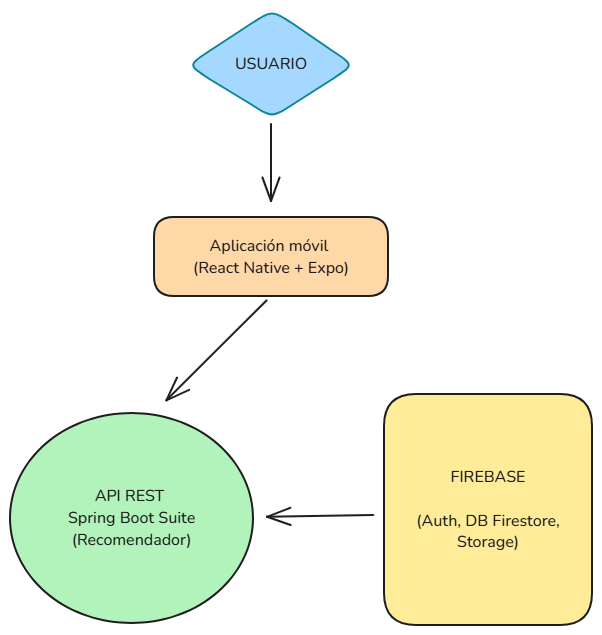
\includegraphics[width = 0.5\textwidth]{Imagenes/esquemas/arq.png}
	\caption{Arquitectura proyecto}
	\label{fig:arquitectura}
\end{figure}

Dada la arquitectura que se puede ver en la (figura \ref{fig:arquitectura}), es importante definir las bases del flujo de la aplicación en cada uno de los procesos.

El usuario abre la aplicación y se encuentra con una pantalla de inicio de sesión/creación de cuenta. En este momento entra en juego Firebase Authentication, lo cual garantiza el acceso a los datos privados del usuario y sus seguridad y sincronización.

Una vez logueado en la aplicación se despliega la página de inicio home desde la cual puede navegar a las diferentes oportunidades que ofrece. 
Por un lado dando al botón de ajustes, tras abrirse un desplegable aparece la opción de cerrar sesión y la de editar el perfil. En el caso de cerrar la sesión se enviará a Firebase la notificación de fin de sesión para seguir manteniendo la privacidad y correcto funcionamiento de la aplicación. 
Por otro lado, en la parte de perfil, se navega a la pantalla perfil, en la cual está definida la foto y de perfil y los demás campos que representan los datos personales del usuario. Desde aquí se pueden realizar las modificaciones y se guardarán automaticamente en la base de datos.

Volviendo a la página de inicio, home, tenemos cuatro opciones principales: hábitos, resultados, calendario y notas, todo ello recogido en una interfaz simple que mantiene los colores del logo.

Todas estas pantallas se encuentran agrupadas por un índice \textbf{(tabs)} que ayuda a gestionar la subapertura de pantallas desde el home.

La pantalla \textbf{Hábitos} se despliega tras pulsar su botón en home. En esta aparece un listado de todas los hábitos que acepta el recomendador con la intención de que el usuario los rellene si es su primera vez haciendolo o carga unos hábitos que tenga almacenados de veces pasadas. De todas formas para una mayor robustez, cada campo cuenta con un manejador de errores que evita introducir datos no reconocibles y lo indica al usuario para que resulte más intuitivo ver donde se encuentran los errores. Tras pulsar en el botón de ejecutar, la aplicación conecta con la API en la cual se encuentra definido el recomendador y que a su vez gestiona la base de datos. De esta forma los datos de hábitos se almacenaran en la base de datos de Firestore y a su vez se ejecutara el recomendador, lo que devuelve una lista de recomondaciones que también se almacenaán y un valor ORI que representa el indice de riesgo de obesidad que se puede inducir de dichos hábitos. 

La pantalla \textbf{Resultados}, se despliega tras pulsar el botón ``Resultados'' en home. En esta pestaña aparece una gráfica similar a un velocímetro que indicará de forma visual los resultados ORI obtenidos por el recomendador. Desde aquí el usuario podra visualizar sus resultados y su lista de recomendaciones producida para poder así empezar una nueva rutina, o gestionar lo máximo posible para obtener la meta.
El objetivo idílico sería ir modificando los hábitos según indiquen las recomendaciones hasta que no quede ninguna recomendación. En ese caso si el ORI sigue siendo más alto de lo deseado, se puede volver a llamar al recomendador, introducir tus nuevos hábitos y solicitar nuevas recomendaciones. Desde esta pantalla ``Resultados'' además de poder ir marcando las recomendaciones completadas, podrás ejecutar la parte del recomendador que actúa como evaluador para ver el progreso. 
Además existe un apartado de ``Historial'' en el cual se pueden ver las últimas modificaciones en los hábitos para de alguna forma incitar al prograso y permitir al usuario ver sus avances.
Volviendo a la parte del recomendador, desde la aplicación se empaquetan los datos en un fichero JSON el cual se envía a la API a través de una petición HTTP POST desarrollada en la propia API en Spring Boot.

La pantalla \textbf{Calendario}, muestra un calendario simple con el cual puedes hacer funciones propias de un calendario, siendo de las más útiles la de poder incluir notas que se guardarán en la base de datos.

La pantalla de \textbf{Notas}, es una gran funcionalidad añadida. En esta pantalla hay un completo gestor de notas con el cual el usuario puede crea, modificar y borrar notas a su prefencia. Estas notas las puede ordendar alfabeticamente por título o por orden de creación, modificación, etc. Con esta funcionalidad el usuario no necesita contar con otra aplicación de gestor de ficheros. Con VitHabitus , no solo obtiene las recomendaciones si no que también puede almacenar rutinas, listas de compra, cambios a realizar en hábitos de forma prograsiva,etc, y todo desde la misma aplicación.

Todas estas ventanas se encuentran vinculadas entre si, por lo que existe un panel inferior que permite una rápida navegación entre ellas sin necesidad de volver a la ventana home, con el objetivo de simplificar las conexiones.

Todo esto desencadena en la existencia de una arquitectura modular y con separación de responsabilidades que permite una gran escalabilidad en caso de querer realizar ampliaciones o extensiones de funciones, como se explica en el apartado CONCLUSIONES Y TRABAJO FUTURO al final de la memoria.


\section{Desarrollo aplicación móvil}

La aplicación ha sido desarrollada a través del editor de código Visual Studio Code, junto con el framework de React Native debido a que es una gran apuesta a la hora de realizar desarrollo de aplicaciones nativas gracias a su simplicidad y su alta compatibilidad de código único válido en multiplataformas. Además se ha usado el entorno Expo el cual es de gran ayuda en la depuración y puesta a punto de la aplicación. Gracias a Expo Go en móviles, con gran facilidad se puede probar la aplicación en el dispositivo en directo, con tan solo escanear el código qr generado por expo.(\cite{ibm_info}). 

Por otro lado los lenguajes más empleados en la elaboración de la aplicación han sido JavaScript para la creación de las pantallas, componentes, etc; y Java para la parte de la API en Spring Boot con el recomendador el cual también se encuentra programado en java.

En esta sección de desarrollo de la aplicación móvil se describe en mayor profundidad el funcionamiento de la applicación pero ya no a nivel de flujo si no a nivel de implementación de código.

Empezamos por la organización del proyecto. La raiz del proyecto app/ constituye el núcleo de la aplicación y en su interior se encuentran difernciadas las distintas pantallas principales y sus componentes reutilizables, así como dato, configuraciones, gestor de navegación...

Como deciamos antes, En primer nivel tenemos la pantalla index.tsx que en React Native es esencial para la indexación de pantallas en la navegación. Login.txs y register.tsx conforman las pantallas de acceso antes de autenticar el usuario. Anidado encontramos el (tabs)/ carpeta la cual incluye las subsecciones de la pantalla home.tsx, página de inicio. Dentro de (tabs)/ encontramos haits.tsx, parte fundamental y núcleo funcional de la aplicación, resultados.tsx, notes.tsx y calendar.tsx. Todas estas páginas responden a un sistema de navegación basado en pestañas (tabs) que facilita al usuario desplazarse.

Por otra parte tenemos los elementos paralelos como los componentes los cuales muchos de ellos son aplicados en las paginas descritas antes. En app/components/ se divin según su potencial uso componentes como casillas, botones con su determinadoestilo, y otros elementos. También hay elementos visuales que conforman la interfaz de usario, la idea es encapsulamiento y modulación para mantener un código más limpio.

Finalmente en lo que respecta a la organización, tenemos la carpeta data/ que recoge todos los archivos de configuración para formularios u otros procesos, como archivos json y datos esenciales. 
Tenemos también la carpeta services/ que recoge todos los fichero s necesarios para la implementación de la APi y de la Firebase; firebaseCOnfig.ts con su configuración de conexión. VerifyApi.ts para su verificación de conexión con la APi en este caso.

No hay que olvidar los ficheros, app.json, eas.json y package.json.
El app.json es el archivo de configuración de expo. Basicamente, recoge el nombre de la aplicación, su logo, requisitos y permisos para que se pueda ejecutar en multiplataforma correctamente. El eas.json, EAS(Expo Application Services) que contiene la información esencial para la realización de builds (app.apk) a través de EXPO,  que sea descargable y ejecutable (la aplicación en formato físico sin necesidad de soporte). Por último el package.json, uno de los más importantes, dado que define las versiones que utilza la aplicación. En caso de no saber que dependencias instalar, e nel package se indican aquellas que son necesarias.

Por otro lado, uno de los elementos más característicos de React Native es el React Navigation que permite realizar las transiciones y navegaciones entre pantallas de forma manual lo que aporta una gran personalización a la aplicación. En el caso de VitHabitus, se hace uso de Expo Router, una herramienta que en este caso genera las rutas de navegación de forma automática basandose en la estrcutura de los archivos del proyecto. 

De esta forma, existen dos archivos layouts uno para app/ y otro para (tabs)/ dado que así cada uno de ellos define el comportamiento y apariencia de las pantallas. (Son como submenus dentro de las subpantallas). De esta forma cada pantalla tiene su ruta bien definida y es más fácil identificar problemas a la hora del testing además de ser más sencillo el añadir nuevas pantallas y secciones.

\subsection{Componentes reutilizables}

Una de las partes más importantes en el desarrollo de una aplicación es la modularidad y el encapsulamiento. Son recursos necesarios para que el código sea lo más legible posible y lo menos repetitivo dado que muchas veces hay fragmentos de código que se repiten en diferentes lugares y que se pueden abstraer. Ese es el caso de las componentes que vamos a ver a continuación.

\begin{itemize}
     \item Entre los componentes más reutilizados se encuentra el \texttt{PickerComponent.tsx} basicamente un selector desplegable que permite a l usuario poder elegir entre diferentes opciones predefinidas. Es uno de los componentes más importantes al ser usado tanto en la creación del formulario para introducir los hábitos y datos en general. La configuración se bada en estructuras de datos externas por lo que es más fácilmente implementable. 

    \item Parecido a el picker encontramos el \textbf{AcordeonHabtis.tsx} usado principalmente en habits.tsx, sirve como un contenedor con la capacidad de plegar y desplegar las secciones, ahorrando mucho espacio visual a la hora de navegar por la pantalla. 
    Cada una de estas secciones se coonstruyen a traves de data/formHabitsStructure.ts que otorga gran flexibilidad al proceso de creación del formulario de hábitos. Es fácilmente modificable añadiendo nuevas secciones en dichgo fichero, sin modificar el componente.

    \item Siguiendo con la parte de texto, destaca el \textbf{FormInput.tsx}, un fichero que se encarga de definir un campo de texto sobre el que poder escribir, se caracteriza por ser modificable con la aplicación de estilos propios y por tener un gran manejo de errores. También header.tsx usado en el login o e HeaderHome.tsxel cual es menos aplicable a otras páginas, ya que representa u header bastante especifico.

    \item Por último a resaltar, a pesar de haber muchos más componentes estos eran los principales. Pero otros componentes visaules como el \textbf{Loader.tsx} el cual es muy útil para gestionar momentos de espera entre navegación de pantallas, cargado y guardado de datos, confirmaciones,etc. El loader.tsx muestra una animación de carga que es muy util y reutilizable en cualquier lugar. De la misma forma el \textbf{CFOmedidor.tsx}, el cual es una representación gráfica de un medidor para indicar el valor del ORI (Obesity Risk Index) de forma clara y visual.
\end{itemize}

En general, el hecho de escribir un programa modular facilita a la hora de modificar, añadir o eliminar elementos.

\subsection{Validación del formulario de Hábitos}

La validación del formulario es esencial para el correcto funcionamiento de la aplicación VitHabitus. La calidad de los datos ha de comprobarse para evitar tener problemas posteriores con el recomendador por valores input no reconocibles. Es por eso que para el desarrollo de esta parte es necesario ser muy minucioso e incorporar un sistema de validación robusto y fiable.

Se basa en una combinación de el fichero \texttt{ValidateHabits.tsx}, el cual evalua la validez de cada campo comprobando que cada uno está dentro de los dominios permitidos. No obstante, además de este fichero es necesario el \texttt{formHabtisStercuture.ts} que mencionamos antes, ya que contiene la definición y estructura concreta de cada una de las secciones y campos. Cuando el usuario introduce un valor, la aplicación evalua en tiempo real ese valor y emite una corrección. Si es válido se acepta pero en caso contrario reproduceun mensaje orientativo para solucionar el error.

Cuando todos los campos son correctos y se puede ejecutar el formulario, se construye un objeto JSON enviable a través de la API mediante una peticion HTTP POST.

\section{Base de datos}

Para la gestión de los datos de la aplicación, VitHabitus utilizada la base de datos NoSql de Firestore, parte de Firbase. Se trata de una base de datos organizada por colecciones y documentos que al formar parte del dominio de Firebase gestiona los datos con gran rendimiento en aplicaciones móviles multiplataforma. Siguiendo con la estructura, para cada usuario se le ha asignado un identificador único que se usa como una llave principal y distintos campos que conforman las subsecciones de cada bloque de datos.

En el caso de los usuarios, la estructura es:
\begin{itemize}
    \item \textbf{Identificador único}. Cada usuario tiene un id único asociado.
    \item \textbf{Colección de hábitos}. Recoge toda la información de los formularios y sus respectivas recomendaciones generadas.
    \item \textbf{Colección de notas}. Son las notas asociadas al usuario. Cuya estrucutra se especifica después.
    \item \textbf{Campo apellido}. Apellido incluido al crear una cuenta de usuario, es modificable.
    \item \textbf{Campo created-at}. Momento de creación del usuario.
    \item \textbf{Campo email}. Correo electrónico introducido al crear una cuenta, es modificable.
    \item \textbf{Campo nombre}. Nombre introducido al crea la cuenta, es modificable.
    \item \textbf{Campo país}. País de nacimiento.
    \item \textbf{Campo teléfono móvil}. Teléfono introducido como posible contaco (opcional), es modificable.
    \item \textbf{Campo imagen}. Foto de perfil (opcional) introducida para personalizar la estática del perfil en la app.
\end{itemize}

Estructura de la subcolección hábitos:
\begin{itemize}
    \item \textbf{formulario}. Recoge todas las variable correspondientes a los hábitos del recomendador, como se puede ver en la sección ``Api Rest- Recomendador Hábitos'' en la memoria. Cuenta también con un campo created-at que permita llevar un historial de creación.
    \item \textbf{Resultados}. Resultados de la recomendación. Lista de modificaciones de las variables de hábitos recomendadas. Cuenta con un created-at para poder llevar contabilidad del momento de creación (historial).
\end{itemize}
Según la configuración, un usuario puede tener un único formulario en activo, un solo conjunto de datos que puede cargar en cualquier momento. No obstante puede tener infinitas recomendaciones y evaluaciones de ese formulario. Por tanto el campo formulario es único pero el de Resultados se gestiona según su identificador y su variable created-at para ordenarlo.

Estructura de la colección de notas:
\begin{itemize}
    \item \textbf{Identificador único}. Cada nota tiene un identificador único asociado que las distingue de las demás.
    \item \textbf{User-id} Identificador del usuario al que está vinculado la nota, al tratarse de una subcolección del usuario.
    \item \textbf{Título de la nota}. Título explicativo de la nota.
    \item \textbf{Contenido}. Texto completo que conforma el cuerpo principal de la nota.
    \item \textbf{Created-at y updated-at}. Campos para llevar la gestión de la creación y actualización de alguno de los campos título o contenido.
\end{itemize}

Para la protección de toda esta información se aplica Firebase Security Rules, que ayuda a el encapsulamiento de los datos, permitiendo que únicamente el usuario concreto pueda acceder a sus propios datos.

En un principio del desarrollo de la aplicación móvil, esta se conectaba directamente con la base de datos. No obstante, tras la creación e implementación de la API todas estas comunicaciones son mediadas a través de la conexión api. Esta solicita al usuario su token de identificador y se lo envía directamente a la Firebase la cual inicia en caso de encontrarse apagada.

Una de las ventajas de Firestore es que cuenta con una gestión automática de una caché local que permite el acceso offline por parte de la aplicación a diferentes contenidos de información.

\section{Autenticación Usuarios}

El sistema de autenticación está basado en el uso del correo electrónico y de la contraseña junto ocn la integración directa de Firebase Authentication.

Firebase Authentication proporciona diferentes funciones siendo las mas importantes, la asignación de un identificador único UID y un control de acceso por fecha y tiempo transcurrido en la app. Además proporciona la posibilidad de establecer la opción de verificar una dirección de correo electrónico para evitar creación masivas de cuentas de usuario falsas con mensajes al correo o via sms. Notificaciones varias e inicio de sesión a través de google, facebook, githug,etc;  y la funcionalidad de restablecer la contraseña en caso de extraviarla.

Estas funcionalidades s ehan implementado en las pantallas \texttt{login.tsx} y \texttt{register.tsx}. Durante el flujo de procesamiento en estas paginas Firebase válida los campos rellenados y comprueba que por ejemplo la contraseña sea lo suficientemente segura. 

La verificación del correo se establece en el fichero \texttt{EmailVerification.tsx} que se encarga de comprobar el correcto funcionamiento de la cuenta de correo y además verifica que el usuario tenga acceso a esta antes de crearla. Para evitar suplantaciones de identidad.

Tras la creación de un usuario y al iniciar sesión, Firebase emite un token de sesión que se mantiene activo hasta que el usuario cierra su sesión. Este token es muy importante para la sincronización y privacidad de la información entre la aplicación y la api y base de datos.


\section{Api Rest}

El sistema de recomendación utilizado en VitHabitus ha sido encapsulado en una API RESTful desarrollada como un servicio independiente gracias al uso del framework Spring Boot. El objetivo de esta API (Interfaz de Programación de Aplicaciones) es implementar el algoritmo del recomendador de la mejor forma posible para la aplicación móvil.(\cite{sts_rest}).
Tras investigar, se llegó a la conclusión de que implementar el algoritmo directamente en la app, provocaria un aumento excesivo del peso y complejidad de esta, provocando ralentizaciones y hasta errores inesperados. Es por ello que finalmente se decidió la realización de una API que posteriormente se encapsularía en un Docker para desplegarla en un servidor propio o en una nube, permitiendo una conexión constante y fluida con la aplicación sin ralentizarla.

La API cuenta con el patrón típico de capas de Spring Boot, con separación de controladores de controladores de entrada, de los modelos que representan las estructuras de datos y de también los servicios que se encargan de procesar la lógica de negocio. De esta manera, el @RestController, también conocido como controlador principal, expone los endpoint como el de tipo POST que recibe el conjunto de hábitos del usuario en formato JSON.

Dada la entrada de datos, se transforman los campos necesarios para poder introducirlos correctamente al recomendador y que este pueda funcionar correctamente. Para ello tenemos el @Service que contiene toda la lógica relacionada con la ejecución del recomendador. Con esto se consigue desacoplar el algoritmo del controlador HTTP.

Con respecto al recomendador, se ha modificado de cierta manera para poder integrarlo lo mejor posible, eliminando toda la capa de interfaz gráfica que tenía. Además hemos divido el reomendador en dos partes: evaluador de hábitos que genera el valor del ORI y busqueda de recomendaciones que realiza todo el proceso para obtener las recomendaciones finales más óptimas.

\subsection{Recomendador de Hábitos}

Entramos en el núcleo funcional de la aplicación VitHabitus, el recomendador de hábitos saludables desarrollado por Fan Ye, Daniel Martínez y recogido en el Trabajo de Fin de Grado: \texttt{``Recomendador de Hábitos para reducir el riesgo
de padecer Sobrepeso y Obesidad''} de la Universidad Complutense de Madrid. (\cite{tfg_recomendador}).

Este algoritmo se fundamenta en la generación de un algoritmo evolutivo, basado en simular procesos que replican la ``selección natural'' para buscar aquellas combinaciones de hábitos más oóptimas.
Este proceso tiene en cuenta una serie de variables inmutables, como la edad, sexo y varaibles modificables como el ejercicio, enfermedades, alimentación, etc.
De esta forma, a partir de los hábitos introducidos, el sistema genera una población inicial de soluciones que se representan como cromosomas. Estos son sometidos a varias iteraciones del ciclo evolutivo con procesos como mutación, cruce, selección, y finalmente la evaluación, a través de una función fitness que representa la calidad de los hábitos en relación con los modelos entrenados.

\begin{figure}[h]
	\centering
	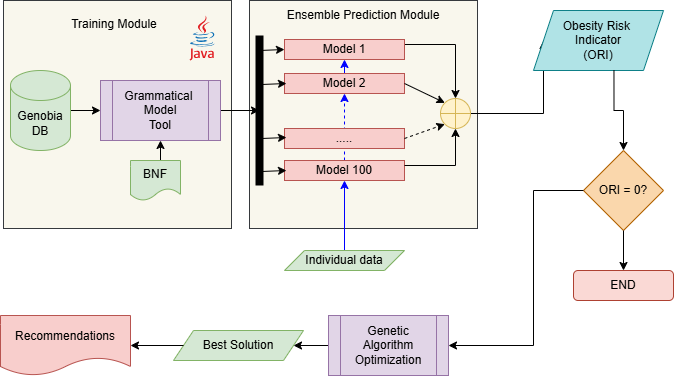
\includegraphics[width = 0.8\textwidth]{Imagenes/esquemas/ObesityRiskIndicator.drawio.png}
	\caption{Arquitectura general del sistema de recomendación}
	\label{fig:Recommendersqueme}
\end{figure}

Se trata de la unificación de dos esquemas presentes en el documento ``An Evolutionary Habit Recommender System to
Reduce the Risk of Overweight and Obesity''.


Para que el recomendador funcione correctamente, uno de los pasos más importantes a realizar, es el uso de los mejores modelos lógicos posibles, los cuales son los encargados de entrenar el algoritmo.
Para ello, el recomendador cuenta con 100 modelos generados a partir de los datos del proyecto \textbf{GenObiA}, una iniciativa multidisciplinar centrada en el análisis del riesgo de obesidad mediante información socio-demográfica, hábitos de la vida y genética de más de 1000 personas.

El sistema se encarga de seleccionar de entre los modelos aquellos que tengan una mayor precisión para ser utilizados en la función fitness de evaluación. Se comparan las distintas soluciones y se selecciona la más prometedora.

Es importante también especificar las distintas variables que son tratadas a lo largo del código del recomendador, las cuales también son declaradas como campos únicos en la colección de formularios de la Base de Datos de Firebase.

Listado de variables:
\begin{enumerate}
    \item \textbf{Sexo}: si la persona es hombre o mujer al nacer.
    \item \textbf{Edad}.
    \item \textbf{Población}: número de personas que viven en la localidad del individuo. Los rangos son: menos de 2.500 habitantes, entre 2.500 y 20.000, entre 20.000 y 50.000 y más de 50.000.
    \item \textbf{Nivel educativo}: puede ser sin estudios, educación primaria, secundaria o universitaria.
    \item \textbf{Ingresos}: situación económica del individuo. Los rangos son: menos de 1.000€ al mes, entre 1.000€ y 2.000€ al mes y más de 2.000€ al mes.
    \item \textbf{Profesión}: tipo de trabajo del individuo, seleccionado de una lista de 16 ocupaciones.
    \item \textbf{Estrés}: si la persona se considera estresada o no.
    \item \textbf{Sueño (8 horas)}: si duerme al menos 8 horas diarias.
    \item \textbf{Bebidas espirituosas}: si consume bebidas alcohólicas fuertes (como licores).
    \item \textbf{Copas de licor}. Número de copas de licor a la semana.
    \item \textbf{Vino o cerveza}: si consume vino o cerveza.
    \item \textbf{Copas de cerveza}. Número de copas de cerveza a la semana.
    \item \textbf{Copas de vino tinto}. Número de copas de vino tinto a la semana.
    \item \textbf{Copas de vino blanco}. Número de copas de vino blanco a la semana.
    \item \textbf{Copas de vino rosado}. Número de copas de vino rosado a la semana.
    \item \textbf{Tabaco}: si fuma cigarrillos actualmente.
    \item \textbf{Número de cigarrillo}. Número de cigarrillos por semana.
    \item \textbf{Pipa}: número de pipas o cargas de pipa que fuma al día.
    \item \textbf{Puros}: número de puros que fuma al día.
    \item \textbf{Años como exfumador}: años desde que dejó de fumar.
    \item \textbf{Exfumador (desconocido)}: si dejó de fumar, pero no sabe desde hace cuánto.
    \item \textbf{Cáncer}: si padece algún tipo de cáncer.
    \item \textbf{Cáncer de mama}.
    \item \textbf{Cáncer de colon}.
    \item \textbf{Cáncer de próstata}.
    \item \textbf{Cáncer de pulmón}.
    \item \textbf{Otros tipos de cáncer}.
    \item \textbf{Infarto de miocardio}.
    \item \textbf{Angina de pecho}.
    \item \textbf{Insuficiencia cardíaca}.
    \item \textbf{Diabetes tipo 2}.
    \item \textbf{Síndrome metabólico}.
    \item \textbf{Apnea del sueño}.
    \item \textbf{Asma}.
    \item \textbf{EPOC}: enfermedad pulmonar obstructiva crónica.
    \item \textbf{Consumo de aceite de oliva}: cucharadas al día.
    \item \textbf{Consumo de verduras}: porciones al día. La guarnición cuenta como media porción.
    \item \textbf{Consumo de frutas}: piezas de fruta al día, incluyendo zumos naturales.
    \item \textbf{Consumo de carne roja}: porciones de carne de vacuno o cerdo al día (hamburguesas, embutidos, fiambres). Cada porción equivale a 100-150g.
    \item \textbf{Consumo de mantequilla o nata}: porciones al día. Cada porción equivale a unos 120g.
    \item \textbf{Consumo de refrescos}: vasos de bebidas azucaradas o carbonatadas al día.
    \item \textbf{Consumo de legumbres}: porciones por semana. Cada porción equivale a 150g.
    \item \textbf{Consumo de pescado o marisco}: porciones por semana. Cada porción equivale a 100-150g o 4-5 piezas de marisco.
    \item \textbf{Consumo de bollería industrial}: veces por semana.
    \item \textbf{Consumo de frutos secos}: porciones por semana. Cada porción equivale a 30g.
    \item \textbf{Consumo de carne blanca}: si prefiere carnes como pollo, pavo o conejo en lugar de carne roja.
    \item \textbf{Consumo de sofritos}: veces que consume sofritos como acompañamiento de pasta, arroz u otros platos por semana.
    \item \textbf{Consumo de lácteos}: veces que consume productos lácteos al día.
    \item \textbf{Lácteos desnatados}: si los productos lácteos consumidos son desnatados o no.
    \item \textbf{EIMS}: minutos semanales de ejercicio intenso.
    \item \textbf{EMMS}: minutos semanales de ejercicio moderado.
    \item \textbf{ECMS}: minutos semanales caminando.
    \item \textbf{Minutos sentado}: tiempo medio que ha pasado sentado durante la última semana.
\end{enumerate}



\section{Tecnologías Utilizadas}

Las principales tecnologías empleadas en este proyecto son las siguiente:
\begin{itemize}
    \item \textbf{Firebase}: Plataforma elegida debido a su amplia gama de servicios y gran compatibilidad con aplicaciones móviles. Se usan principalmente los servicios de Atutenticación de usuarios para la gestión de los usuarios y Firestore para el almacenamiento de datos en la nube.(\cite{firebase_docs}) 
    \item \textbf{React Native}: Framework empleado para el desarrollo de la parte frontend, interfaz de la aplicación VitHabitus. Destaca por la facilidad de crear aplicaciones tanto para Andorid como para iOS en un mismo proyecto. Además de ofrecer similitudes con estilos como css y ser un framework sencillo e intuitivo para aquellos desarrolladores primerizos. Esto se debe gracias a sus librerias que facilitan en gran medida las conexiones backend como a una API o Base de Datos. React native, Calendars, compatibilidad con Expo, etc. (\cite{react_native})
    \item \textbf{Expo}: Entorno de desarrollo utilizado para aplicaciones móviles basadas en React Native. Expo proporciona una experiencia completa en la craeción prueba y despliegue de una aplicación en diferentes dispositivos móviles android y iOS, gacias a sus numerosas herramientas que resultan de gran utilidad. 
    Aplicaciones como Expo GO que permiten previsualizar la app en tiempo real desde un dispositivo físico sin compilar el proyecto. Eas de Expo(\cite{eas}) que permite la generación de binarios, builds listos para la instalación o publicación. Librerias como Expo router que implementan de forma sencilla la navegación entre pantallas basandose en la estructura de archvios y haciendo el proyecto más escalable. Entre otras.(\cite{expo_docs})
    \item \textbf{NodeJS}: Es un entorno de ejecución para JavaScript. Se utilzia en el proyecto como base para el entorno de desarrollo de React native, sinedo su función principal permitir la ejecución de herramientas y scripts que son necesarias para que la aplicación funcione. Tiene además herramientas como Express para la cración de API-Rest.(\cite{nodejs})
    \item \textbf{NPM (Node Package Manager}: Es un gestor de paquetes asociado al escosistema de JavaScript. NPM es imprescindible en el funcionamiento de la app, siendo el comando ``npm install'' necesario siempre para confirmar la instalación de todas las dependencias correctas y necesarias. Tiene scripts definidos muy útiles en el archivo package.json que automatizan varios procesos.
    \item \textbf{TypeScript}: Es preferible su uso sobre JavaScript debido a su tipado estático, lo que garantiza mayor seguridad y claridad en el código. Especialmente para desarrolladores acostumbrados a lenguajes tipados. 
    \item \textbf{Github y git}: Para el control de versiones y modificaciones del código se ha utilizado la herramienta git junto con la interzad de github con el uso de un repositorio.
    \item \textbf{Spring Boot Suite}: Se trata de un entorno de desarrollo integrado basado en eclipse que se utiliza en la creación de la API REST. Es muy utilizado para construir servicios web de forma rápida, modular y con las configuraciones necesarias. Tiene gran valor gracias a su compatibilidad con Maven(gestión de dependencias, archivo pom.xml) y Java, lenguaje en el que está implementado e recomendador.(\cite{sts}).
\end{itemize}

%\include{Capitulos/Capitulo4}
%\include{Capitulos/Capitulo5}
\chapter{Conclusiones y Trabajo Futuro}
\label{cap:conclusiones}

Conclusiones del trabajo y líneas generales de trabajo futuro.

Teniendo encuenta el proceso completo, el desarrollo de VitHabitus ha supuesto un reto técnico e interesante al ser mi presentación al mundo de las aplicaciones móviles. 

Al final se ha conseguido cumplir gran parte de los objetivos propuestos, con el desarrollo del frontend y el backend con la API y la base de datos de Firebase.
Integración del algoritmo de recomendación de hábitos y un correcto flujo de funcionamiento entre todos los elementos.

Queda como resultado una aplicación que supone de gran utilidad para muchas personas y que demuestra una vez más, el increible potencial que tiene la inteligencia artificial aplicada a la salud. Además demuestra como el desarrollo de aplicaciones móviles puede actuar como un canal eficaz para trasladar tecnologías complejas a la vida cotidiana de las personas, gracias a una interfaz intuitiva y de fácil uso a través de un teléfono móvil.

\subsection{Trabajo Futuro}

Independientemente del resultado. Siempre hay posibilidad de mejora y avances. 
De esta forma, hay algunos ideas que surgieron durante la realización del proyecto.
Una de las más importantes sería la ampliación del formulario de hábitos, permitiendo ser aún más flexible con más hábitos que representen relación con la obesidad. 

\begin{itemize}
    \item Implementación de conectividad con dispositivos wearables que contienen sensores que podrían calcular datos como pulsaciones, horas de sueño, calorias quemadas, que pueden ser de gran utilidad para el recomendador.
    \item Publicar la aplicación de forma oficial en google play y App Store, lo que supondría cumplir con los estandares solicitados y mantener la aplicación actualizada
    \item Traducir la aplicación a varios idiomas o al menos al inglés para tener futuro en el mercado internacional. 
    \item Por otro lado en la parte visual, hay ciertos partes que se podrían mejorar para obtener un acabado más profesional.
\end{itemize}

. 





%%%%%%%%%%%%%%%%%%%%%%%%%%%%%%%%%%%%%%%%%%%%%%%%%%%%%%%%%%%%%%%%%%%%%%%%%%%
% Si el TFG se escribe en inglés, comentar las siguientes líneas 
% porque no es necesario incluir nuevamente las Conclusiones en inglés
\begin{otherlanguage}{english}
\chapter*{Conclusions and Future Work}
\label{cap:conclusions}
\addcontentsline{toc}{chapter}{Conclusions and Future Work}

Conclusions and future lines of work. This chapter contains the translation of Chapter \ref{cap:conclusiones}.

Taking into account the entire process, the development of VitHabitus has been a technical and a rewarding challenge, as it was my first step into the world of mobile applications.

In the end, most of the initial objectives were successfully achieved, including the development of both the frontend and backend, the implementation of the API and the integration with Firebase as the database. The habit recommendation algorithm was also successfully incorporated, resulting in a coherent and functional flow between all components.

The final product is an application that can be highly useful for many users and it clearly showcases the incredible potential of artificial intelligence when applied to health. Also, it demonstrates how mobile app development can serve as an effective channel for bringing complex technologies into people's everyday lives, thanks to an intuitive and easy-to-use interface accessible from any smartphone

\subsection*{Future Work}

Regardless of the current outcome, there is always room for improvement and growth.
Some ideas emerged throughout the development process and some of the mos relevant are this ones:
\begin{itemize}
    \item Implement connectivity with wearable devices equipped with sensors that could track valuable data such as heart rate, sleep duration, calories burned... variables that could been applied to the recommendation system.
    \item Officially publish the app on Google Play and Apple Store, which involve setting the required standards and ensuring continuous updates.
    \item Translating the app into multiple languages, or at least into English, to increase its potential to reach the international market.
    \item In the visual aspects, improving some aspects of the user interface to achieve more polished and visual finish.
\end{itemize}


\end{otherlanguage}
%%%%%%%%%%%%%%%%%%%%%%%%%%%%%%%%%%%%%%%%%%%%%%%%%%%%%%%%%%%%%%%%%%%%%%%%%%%

\include{Capitulos/ContribucionesPersonales}

%
% Bibliografía
%
% Si el TFM se escribe en inglés, editar TeXiS/TeXiS_bib para cambiar el
% estilo de las referencias
%---------------------------------------------------------------------
%
%                      configBibliografia.tex
%
%---------------------------------------------------------------------
%
% bibliografia.tex
% Copyright 2009 Marco Antonio Gomez-Martin, Pedro Pablo Gomez-Martin
%
% This file belongs to the TeXiS manual, a LaTeX template for writting
% Thesis and other documents. The complete last TeXiS package can
% be obtained from http://gaia.fdi.ucm.es/projects/texis/
%
% Although the TeXiS template itself is distributed under the 
% conditions of the LaTeX Project Public License
% (http://www.latex-project.org/lppl.txt), the manual content
% uses the CC-BY-SA license that stays that you are free:
%
%    - to share & to copy, distribute and transmit the work
%    - to remix and to adapt the work
%
% under the following conditions:
%
%    - Attribution: you must attribute the work in the manner
%      specified by the author or licensor (but not in any way that
%      suggests that they endorse you or your use of the work).
%    - Share Alike: if you alter, transform, or build upon this
%      work, you may distribute the resulting work only under the
%      same, similar or a compatible license.
%
% The complete license is available in
% http://creativecommons.org/licenses/by-sa/3.0/legalcode
%
%---------------------------------------------------------------------
%
% Fichero  que  configura  los  parámetros  de  la  generación  de  la
% bibliografía.  Existen dos  parámetros configurables:  los ficheros
% .bib que se utilizan y la frase célebre que aparece justo antes de la
% primera referencia.
%
%---------------------------------------------------------------------


%%%%%%%%%%%%%%%%%%%%%%%%%%%%%%%%%%%%%%%%%%%%%%%%%%%%%%%%%%%%%%%%%%%%%%
% Definición de los ficheros .bib utilizados:
% \setBibFiles{<lista ficheros sin extension, separados por comas>}
% Nota:
% Es IMPORTANTE que los ficheros estén en la misma línea que
% el comando \setBibFiles. Si se desea utilizar varias líneas,
% terminarlas con una apertura de comentario.
%%%%%%%%%%%%%%%%%%%%%%%%%%%%%%%%%%%%%%%%%%%%%%%%%%%%%%%%%%%%%%%%%%%%%%
\setBibFiles{%
biblio%
}

%%%%%%%%%%%%%%%%%%%%%%%%%%%%%%%%%%%%%%%%%%%%%%%%%%%%%%%%%%%%%%%%%%%%%%
% Definición de la frase célebre para el capítulo de la
% bibliografía. Dentro normalmente se querrá hacer uso del entorno
% \begin{FraseCelebre}, que contendrá a su vez otros dos entornos,
% un \begin{Frase} y un \begin{Fuente}.
%
% Nota:
% Si no se quiere cita, se puede eliminar su definición (en la
% macro setCitaBibliografia{} ).
%%%%%%%%%%%%%%%%%%%%%%%%%%%%%%%%%%%%%%%%%%%%%%%%%%%%%%%%%%%%%%%%%%%%%%
\setCitaBibliografia{
\begin{FraseCelebre}
\begin{Frase}
  Y así, del mucho leer y del poco dormir, se le secó el celebro de
  manera que vino a perder el juicio.\\ 
\end{Frase}
\begin{Fuente}
  Miguel de Cervantes Saavedra
\end{Fuente}
\end{FraseCelebre}
}

%%
%% Creamos la bibliografia
%%
\makeBib

% Variable local para emacs, para  que encuentre el fichero maestro de
% compilación y funcionen mejor algunas teclas rápidas de AucTeX

%%%
%%% Local Variables:
%%% mode: latex
%%% TeX-master: "../Tesis.tex"
%%% End:



% Apéndices
\appendix
%\include{Apendices/appendixA}
%\include{Apendices/appendixB}
%\include{Apendices/appendixC}
%\include{...}
%\include{...}
%\include{...}
\backmatter



%
% Índice de palabras
%

% Sólo  la   generamos  si  está   declarada  \generaindice.  Consulta
% TeXiS.sty para más información.

% En realidad, el soporte para la generación de índices de palabras
% en TeXiS no está documentada en el manual, porque no ha sido usada
% "en producción". Por tanto, el fichero que genera el índice
% *no* se incluye aquí (está comentado). Consulta la documentación
% en TeXiS_pream.tex para más información.
\ifx\generaindice\undefined
\else
%%---------------------------------------------------------------------
%
%                        TeXiS_indice.tex
%
%---------------------------------------------------------------------
%
% TeXiS_indice.tex
% Copyright 2009 Marco Antonio Gomez-Martin, Pedro Pablo Gomez-Martin
%
% This file belongs to TeXiS, a LaTeX template for writting
% Thesis and other documents. The complete last TeXiS package can
% be obtained from http://gaia.fdi.ucm.es/projects/texis/
%
% This work may be distributed and/or modified under the
% conditions of the LaTeX Project Public License, either version 1.3
% of this license or (at your option) any later version.
% The latest version of this license is in
%   http://www.latex-project.org/lppl.txt
% and version 1.3 or later is part of all distributions of LaTeX
% version 2005/12/01 or later.
%
% This work has the LPPL maintenance status `maintained'.
% 
% The Current Maintainers of this work are Marco Antonio Gomez-Martin
% and Pedro Pablo Gomez-Martin
%
%---------------------------------------------------------------------
%
% Contiene  los  comandos  para  generar  el índice  de  palabras  del
% documento.
%
%---------------------------------------------------------------------
%
% NOTA IMPORTANTE: el  soporte en TeXiS para el  índice de palabras es
% embrionario, y  de hecho  ni siquiera se  describe en el  manual. Se
% proporciona  una infraestructura  básica (sin  terminar)  para ello,
% pero  no ha  sido usada  "en producción".  De hecho,  a pesar  de la
% existencia de  este fichero, *no* se incluye  en Tesis.tex. Consulta
% la documentación en TeXiS_pream.tex para más información.
%
%---------------------------------------------------------------------


% Si se  va a generar  la tabla de  contenidos (el índice  habitual) y
% también vamos a  generar el índice de palabras  (ambas decisiones se
% toman en  función de  la definición  o no de  un par  de constantes,
% puedes consultar modo.tex para más información), entonces metemos en
% la tabla de contenidos una  entrada para marcar la página donde está
% el índice de palabras.

\ifx\generatoc\undefined
\else
   \addcontentsline{toc}{chapter}{\indexname}
\fi


% Generamos el índice
\printindex

% Variable local para emacs, para  que encuentre el fichero maestro de
% compilación y funcionen mejor algunas teclas rápidas de AucTeX

%%%
%%% Local Variables:
%%% mode: latex
%%% TeX-master: "./tesis.tex"
%%% End:

\fi

%
% Lista de acrónimos
%

% Sólo  lo  generamos  si  está declarada  \generaacronimos.  Consulta
% TeXiS.sty para más información.


\ifx\generaacronimos\undefined
\else
%---------------------------------------------------------------------
%
%                        TeXiS_acron.tex
%
%---------------------------------------------------------------------
%
% TeXiS_acron.tex
% Copyright 2009 Marco Antonio Gomez-Martin, Pedro Pablo Gomez-Martin
%
% This file belongs to TeXiS, a LaTeX template for writting
% Thesis and other documents. The complete last TeXiS package can
% be obtained from http://gaia.fdi.ucm.es/projects/texis/
%
% This work may be distributed and/or modified under the
% conditions of the LaTeX Project Public License, either version 1.3
% of this license or (at your option) any later version.
% The latest version of this license is in
%   http://www.latex-project.org/lppl.txt
% and version 1.3 or later is part of all distributions of LaTeX
% version 2005/12/01 or later.
%
% This work has the LPPL maintenance status `maintained'.
% 
% The Current Maintainers of this work are Marco Antonio Gomez-Martin
% and Pedro Pablo Gomez-Martin
%
%---------------------------------------------------------------------
%
% Contiene  los  comandos  para  generar  el listado de acrónimos
% documento.
%
%---------------------------------------------------------------------
%
% NOTA IMPORTANTE:  para que la  generación de acrónimos  funcione, al
% menos  debe  existir  un  acrónimo   en  el  documento.  Si  no,  la
% compilación  del   fichero  LaTeX  falla  con   un  error  "extraño"
% (indicando  que  quizá  falte  un \item).   Consulta  el  comentario
% referente al paquete glosstex en TeXiS_pream.tex.
%
%---------------------------------------------------------------------


% Redefinimos a español  el título de la lista  de acrónimos (Babel no
% lo hace por nosotros esta vez)

\def\listacronymname{Lista de acrónimos}

% Para el glosario:
% \def\glosarryname{Glosario}

% Si se  va a generar  la tabla de  contenidos (el índice  habitual) y
% también vamos a  generar la lista de acrónimos  (ambas decisiones se
% toman en  función de  la definición  o no de  un par  de constantes,
% puedes consultar config.tex  para más información), entonces metemos
% en la  tabla de contenidos una  entrada para marcar  la página donde
% está el índice de palabras.

\ifx\generatoc\undefined
\else
   \addcontentsline{toc}{chapter}{\listacronymname}
\fi


% Generamos la lista de acrónimos (en realidad el índice asociado a la
% lista "acr" de GlossTeX)

\printglosstex(acr)

% Variable local para emacs, para  que encuentre el fichero maestro de
% compilación y funcionen mejor algunas teclas rápidas de AucTeX

%%%
%%% Local Variables:
%%% mode: latex
%%% TeX-master: "../Tesis.tex"
%%% End:

\fi

%
% Final
%
%---------------------------------------------------------------------
%
%                      fin.tex
%
%---------------------------------------------------------------------
%
% fin.tex
% Copyright 2009 Marco Antonio Gomez-Martin, Pedro Pablo Gomez-Martin
%
% This file belongs to the TeXiS manual, a LaTeX template for writting
% Thesis and other documents. The complete last TeXiS package can
% be obtained from http://gaia.fdi.ucm.es/projects/texis/
%
% Although the TeXiS template itself is distributed under the 
% conditions of the LaTeX Project Public License
% (http://www.latex-project.org/lppl.txt), the manual content
% uses the CC-BY-SA license that stays that you are free:
%
%    - to share & to copy, distribute and transmit the work
%    - to remix and to adapt the work
%
% under the following conditions:
%
%    - Attribution: you must attribute the work in the manner
%      specified by the author or licensor (but not in any way that
%      suggests that they endorse you or your use of the work).
%    - Share Alike: if you alter, transform, or build upon this
%      work, you may distribute the resulting work only under the
%      same, similar or a compatible license.
%
% The complete license is available in
% http://creativecommons.org/licenses/by-sa/3.0/legalcode
%
%---------------------------------------------------------------------
%
% Contiene la última página
%
%---------------------------------------------------------------------


% Ponemos el marcador en el PDF
\ifpdf
   \pdfbookmark{Fin}{fin}
\fi

\thispagestyle{empty}\mbox{}

\vspace*{4cm}

\small

\hfill \emph{--¿Qué te parece desto, Sancho? -- Dijo Don Quijote --}

\hfill \emph{Bien podrán los encantadores quitarme la ventura,}

\hfill \emph{pero el esfuerzo y el ánimo, será imposible.}

\hfill 

\hfill \emph{Segunda parte del Ingenioso Caballero} 

\hfill \emph{Don Quijote de la Mancha}

\hfill \emph{Miguel de Cervantes}

\vfill%space*{4cm}

\hfill \emph{--Buena está -- dijo Sancho --; fírmela vuestra merced.}

\hfill \emph{--No es menester firmarla -- dijo Don Quijote--,}

\hfill \emph{sino solamente poner mi rúbrica.}

\hfill 

\hfill \emph{Primera parte del Ingenioso Caballero} 

\hfill \emph{Don Quijote de la Mancha}

\hfill \emph{Miguel de Cervantes}


\newpage
\thispagestyle{empty}\mbox{}

\newpage

% Variable local para emacs, para  que encuentre el fichero maestro de
% compilación y funcionen mejor algunas teclas rápidas de AucTeX

%%%
%%% Local Variables:
%%% mode: latex
%%% TeX-master: "../Tesis.tex"
%%% End:

%\end{otherlanguage}
\end{document}
